\documentclass[12pt]{article}


\title{Power-Index Game Research Write-up}
\date{Aug 2018}
\author{Charlie Gerrie}
\usepackage[utf8]{inputenc}


\usepackage{amsthm}
\usepackage{amsmath}
\usepackage{yfonts}
\usepackage{amssymb}
\usepackage{fullpage}
\usepackage{mathtools}
\usepackage{tikz}
\usepackage{graphicx}
\usepackage{subcaption}
\usepackage{float}
\usepackage{pgf}
\usetikzlibrary{arrows}
\DeclarePairedDelimiter\ceil{\lceil}{\rceil}
\DeclarePairedDelimiter\floor{\lfloor}{\rfloor}
\pagestyle{empty}

\newtheorem{theorem}{Theorem}%[section]

\newtheorem{lemma}{Lemma}%[section]

\newtheorem{proposition}{Proposition}%[section]

\newtheorem{corollary}{Corollary}%[section]

\theoremstyle{definition}
\newtheorem{definition}{Definition}%[section]
 
\theoremstyle{remark}
\newtheorem{remark}{Remark}%[section]

\theoremstyle{remark}
\newtheorem{example}{Example}%[section]

\pagenumbering{gobble}
% TODO SHOULD I HAVE PAGE NUMBERS?

\begin{document}

%TITLE PAGE%
\maketitle
\newpage

\begin{abstract}
We examine the power-index game, a cellular automaton, on a torus. 
\end{abstract}

\tableofcontents

\section{Introduction} \label{IntroSec}

\subsection{The Power Index Game} \label{PIgame}

% explain that it's played on a graph
% define sides (WEAK/STRONG)
% define closed neighborhood
% define together and against sets
% define power
% define iteration behaviour
% explain iteration
\begin{definition}[Side]
We define the set of sides $\mathbb{S}$ to be the set containing two elements $\mathfrak{s}$ and $\mathfrak{w}$. \textit{These sides will also be associated with and referred to by the colours black and white}.
\end{definition}

\begin{definition}[Game]
A game $G(B,S)$ is a structure composed of both a graph $B(V,E)$ (as in board) with associated vertex and edge sets $V$ and $E$, and a mapping $S\colon V \to \mathbb{S}$, which assigns a side to each vertex.
\end{definition}

\begin{definition}[Iteration operator]
We define an operator $I$ which acts on a game to iterate it. For example, $IG$ would be the game $G$ iterated once, and $I^n G$ would be it iterated $n$ times.
\end{definition}

\subsection{Prior Work and Variations} \label{PriorWork}

% talk with Jordan

\subsection{Improvements on Prior Results} \label{Improvements}
% ARBITRARY CYCLES (SHOULD THIS BE IN THE "POWER INDEX ON A TORUS" SECTION?)
% motivate arbitrary cycles
\par
Recall that one of the previous results was arbitrarily large cycles. This raises the question of if cycles of any specific length can occur in the game. We have found a construction that demonstrates that this is possible.
% show initial conditions for astakos
\par
Consider the following configuration on a torus % smallest astakos
This construction can be generalized to a $3\times n$ torus which corresponds to a cycle length of $n$. 
% show that it iterates and loops (make sure you mention that it's on a torus)
% result: arbitrary cycles are possible

\section{The Power Index Game on a Torus} \label{Main Chapter}
%mention toroidal grid
\subsection{Simplifications}
% motivation
The rules of the game can be restated in simpler terms when limited to a torus. All of the tori we have used have been toroidal grids, so the graphs are 4-regular. Thus, the rules from \ref{PIgame} for the power can be simplified to a simple 1-neighborhood cellular automaton with the following rules:
% definitions
% power
\begin{equation}
	P(v) =
	\begin{cases}
		\frac{1}{3} & \text{if $|A(v)|=2$} \\
		\frac{1}{4} & \text{if $|A(v)|=3$} \\
		\frac{1}{5} & \text{if $|A(v)|=4$} \\
		0 & \text{if $|A(v)|\in \{0,1\}$}
	\end{cases}
\end{equation}
% next iteration?
	
% results
	% explain 2-neighborhood
	
% % % % SYMMETRIES!
\subsection{Symmetries}

% SIDE
% ROTATIONAL
% TRANSLATIONAL

\subsection{Examples}

% help people get a sense of how the game goes

\subsection{Special Shapes} \label{SpecialShapes}

\par

% motivation

\begin{definition}[Configuration]
A configuration is a state of an entire graph.
\end{definition}
% EXAMPLES

\begin{definition}[Subconfiguration]
A subconfiguration is an arrangement of cells, irrespective of its surrounding configuration.
\end{definition}
% EXAMPLES

% results of these definitions

\subsubsection{On An Empty Grid} \label{EmptyGrid}
\par
These shapes are considered to be simulated on a grid of entirely the opposite colour, devoid of any other patterns.

\begin{definition}[Unstable Subconfiguration]
A configuration is called unstable if there exists a finite number of iterations after which it will die out, and the grid returns to homogeneity. 
\end{definition}
\begin{example}
A chevron is an unstable subconfiguration, since it dies out after two iterations.

%FIGURES

\end{example}


\begin{definition}[Stable Subconfiguration]
A configuration is called stable if there exists a finite number of iterations after which it will be reproduced. 
\end{definition}
\begin{example}
A 3-by-3 square is a stable subconfiguration, since if it is placed in a field of the opposite colour it will form a cycle of length 3. See figure \ref{StableConfigs}.

\begin{figure}
  \centering
  \begin{subfigure}[b]{0.2\linewidth}
    
\includegraphics[width=\linewidth]{3x3_1.png}
    \caption{Iteration 1}
    \label{fig:3x3_1}
  \end{subfigure}
  \begin{subfigure}[b]{0.2\linewidth}
    
\includegraphics[width=\linewidth]{3x3_2.png}
    \caption{Iteration 2}
    \label{fig:3x3_2}
  \end{subfigure}
  \begin{subfigure}[b]{0.2\linewidth}
    
\includegraphics[width=\linewidth]{3x3_3.png}
    \caption{Iteration 3}
    \label{fig:3x3_3}
  \end{subfigure}
  \begin{subfigure}[b]{0.2\linewidth}
    
\includegraphics[width=\linewidth]{3x3_1.png}
    \caption{Iteration 4}
    \label{fig:3x3_4}
  \end{subfigure}
  \caption{3-by-3 square on a 12-by-12 torus}
  \label{StableConfigs}
\end{figure}



%FIGURES

\end{example}
\begin{remark}
The 5-by-5 and 7-by-7 square are also stable. This sparked the idea that maybe all odd squares above 2 were stable. This hypothesis was quickly disproven by considering the 9-by-9 square, which is parastable.
\end{remark}

\begin{definition}[Parastable Subconfiguration]
A configuration is called parastable if it doesn't die out, but instead fills its space with stable patterns.
\end{definition}
\begin{example}
A 2-by-2 square is a parastable subconfiguration. See figure \ref{ParastableFig}.

\begin{figure}[H]
  \centering
  \begin{subfigure}[b]{0.25\linewidth}
    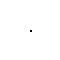
\includegraphics[width=\linewidth]{2x2_1.png}
    \caption{Iteration 1}
    \label{fig:2x2_1}
  \end{subfigure}
  \begin{subfigure}[b]{0.25\linewidth}
    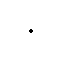
\includegraphics[width=\linewidth]{2x2_2.png}
    \caption{Iteration 2}
    \label{fig23x2_2}
  \end{subfigure}
  \begin{subfigure}[b]{0.25\linewidth}
    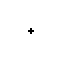
\includegraphics[width=\linewidth]{2x2_3.png}
    \caption{Iteration 3}
    \label{fig:2x2_3}
  \end{subfigure}
  \begin{subfigure}[b]{0.25\linewidth}
    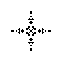
\includegraphics[width=\linewidth]{2x2_20.png}
    \caption{Iteration 20}
    \label{fig:2x2_20}
  \end{subfigure}
  \begin{subfigure}[b]{0.25\linewidth}
    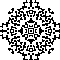
\includegraphics[width=\linewidth]{2x2_50.png}
    \caption{Iteration 50}
    \label{fig:2x2_50}
  \end{subfigure}
  \begin{subfigure}[b]{0.25\linewidth}
    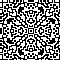
\includegraphics[width=\linewidth]{2x2_100.png}
    \caption{Iteration 100}
    \label{fig:2x2_100}
  \end{subfigure}
  \caption{2-by-2 square on a 60-by-60 torus}
  \label{ParastableFig}
\end{figure} 

\end{example}
\begin{example}
Consider the tetrominoes. All subconfigurations with less than four cells are unstable, so these are the first ones to exhibit parastability. Though the S, Z, and T tetrominoes are unstable, the L, I, and O tetrominoes are all parastable. % DIAGRAMS OF THEM
\begin{figure}[H]
  \centering
  \begin{subfigure}[b]{0.4\linewidth}
    \fbox{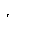
\includegraphics[width=\linewidth]{Lstart.png}}
    \caption{iteration 1}
  \end{subfigure}
  \begin{subfigure}[b]{0.4\linewidth}
    \fbox{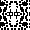
\includegraphics[width=\linewidth]{Lend.png}}
    \caption{iteration 93}
  \end{subfigure}
  \caption{L tetromino}
\end{figure}
\end{example}

\par
Not much is understood about the mechanism of parastability at this time. However, for large subconfigurations, it appears that stability or unstability are the exceptions whereas parastability is the rule.

\subsubsection{A Glider}
\par
We have discovered a construction to have a cycle of arbitrary length greater or equal to 6. See figure \ref{Astakos}.

% DIAGRAM SHOWING POWERS

\begin{figure}[H]
  \centering
  \begin{subfigure}[b]{0.25\linewidth}
    \fbox{
\includegraphics[width=\linewidth]{astakos1.png}}
    \caption{Iteration 1}
  \end{subfigure}
  \begin{subfigure}[b]{0.25\linewidth}
    \fbox{
\includegraphics[width=\linewidth]{astakos2.png}}
    \caption{Iteration 2}
  \end{subfigure}
  \begin{subfigure}[b]{0.25\linewidth}
    \fbox{
\includegraphics[width=\linewidth]{astakos3.png}}
    \caption{Iteration 3}
  \end{subfigure}
  \begin{subfigure}[b]{0.25\linewidth}
    \fbox{
\includegraphics[width=\linewidth]{astakos4.png}}
    \caption{Iteration 4}
  \end{subfigure}
  \begin{subfigure}[b]{0.25\linewidth}
    \fbox{
\includegraphics[width=\linewidth]{astakos5.png}}
    \caption{Iteration 5}
  \end{subfigure}
  \begin{subfigure}[b]{0.25\linewidth}
    \fbox{
\includegraphics[width=\linewidth]{astakos6.png}}
    \caption{Iteration 6}
  \end{subfigure}
  \begin{subfigure}[b]{0.25\linewidth}
    \fbox{
\includegraphics[width=\linewidth]{astakos1.png}}
    \caption{Iteration 7}
  \end{subfigure}
  \caption{The glider}
  \label{Astakos}
\end{figure}

\begin{theorem}
The power-index game is capable of having arbitrary cycles.
\end{theorem}
\begin{proof}
Cycles of length 1 through 5 are trivial. All larger cycles of length $n$ can be constructed by placing a glider on a $3$-by-$n$ board.
\end{proof}
\begin{remark}
We dubbed the glider "\textit{astakos}", after the greek work for lobster.
\end{remark}

\subsubsection{Uniform Power Configurations} \label{UPCs} %ACTUALLY USE THIS ACCRONYM?
\begin{definition}[Uniform Power Configuration (UPC)]
A configuration where every cell has the same power.
\end{definition}
\par
We consider UPCs because they will always be static; For a cell to change it would have to have a more powerful neighbor. On a torus, there are four options for the power of a cell: $0$, $\frac{1}{3}$, $\frac{1}{4}$, and $\frac{1}{5}$. % CHECK "HAVE" SYNTAX -_-

\par
The first of these which we will consider is configurations with a uniform power of $\frac{1}{5}$, since they are the simplest. For a cell to have a power of $\frac{1}{5}$, it must be surrounded entirely by neighbors of its own side. Thus, such configurations must be made up of entirely one colour. This type of configuration can be made on a torus of any dimensions.

\par
% rewrite this as opposing or opposite side?
Next, we will consider those with a power of $\frac{1}{4}$. In this case, every cell must have one neighbor of the opposite side. Thus, we can inductively construct what this configuration will look like by starting with a single cell.
% FIGURE OF A CELL WITH A 1-NEIGHBORHOOD WITH ALL BUT THE RIGHT CELL BEING THE WHITE
% LABEL THE RIGHT ONE R, AND THE ONES ABOVE AND BELOW R AS a AND b
\begin{figure}[H]
	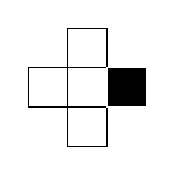
\begin{tikzpicture}
		\draw(0,0.5) rectangle (0.5,1);
		\draw(0.5,0) rectangle (1,0.5);
		\draw(0.5,0.5) rectangle (1,1);					% REPEAT ME!
		\draw(0.5,1) rectangle (1,1.5);
		\path[draw=white,fill=black] (1,0.5) rectangle (1.5,1);
	\end{tikzpicture}
\end{figure}
Now, we know that the spaces to at $a$ and $b$ must be the same side as $R$, because if they were not, then $R$ would have two neighbors of the opposite side.
\\
FIGURE WITH a AND b FILLED IN, AND THE CELLS ABOVE IT AND TO ITS LEFT LABELED c AND d
\\
Now we see that $c$ and $d$ must be coloured the same colour as the cells below them. We can continue this type of argument upwards and downwards, forming stripes.
% FIGURE OF TWO ADJACENT 2-STRIPES WITH DOMAINS LEFT AND RIGHT LABELLED L AND R
\\
Finally, we see that the domains $L$ and $R$ must be black and white. Thus, we can continue this pattern to the left and right.
% FINAL FIGURE
We call this pattern a tessellation of 2-stripes, since each stripe is two cells wide. This configuration has a limitation on its dimensions. In this case, the width must be a multiple of 4 to accommodate the repeating pattern of the 2-stripes. So, for example, a UPC could not exist on a 3-by-5 torus, but one could exist on a 3-by-4 torus. On tori where both dimensions are multiples of 4, the stripes can be placed in either orientation.

\par
% UPC OF 0 POWER
UPCs of power $0$ are somewhat more complicated than the previous ones. First off, the trivial solution to having a board with uniform power $0$ is a checkerboard pattern, where every cell has zero neighbors on its side. Note that checkerboard configurations can only exist on even-by-even tori.
\begin{figure}[H]
  \centering
  \fbox{
\includegraphics[width=0.5\linewidth]{checkers.png}}
  \caption{Checkerboard}
\end{figure}
\par
However, cells will also have power $0$ if they have one neighbor on the same side. In this case, we can use the inductive method we used for $\frac{1}{4}$-power. Start with a single cell.
% DIAGRAM OF SINGLE CELL WITH UPPER, LEFT, AND BELOW CELLS THE OPPOSITE COLOUR. LABEL CENTRE S AND RIGHT CELL a
Next we can fill in the neighbors of $a$.
% DIAGRAM WITH RIGHT CELL NEIGHBORHOOD FILLED IN. LABEL TWO TOP CELLS b AND c, BOTTOM d AND e
Now we recognize that the pairs of $b$ and $c$, and $d$ and $e$, are just like the pair $S$ and $a$. Thus, we can continue the pattern up and down arbitrarily. This forms an alternating stripe 2 cells wide. The beauty of such a stripe is that the sides of it can fit into an existing checkerboard pattern.
\begin{theorem}
There cannot be both horizontal and vertical stripes on a $0$-power UPC.
\end{theorem}
\begin{proof}
Suppose you could have both. They would intersect somewhere, which would break the extending-upwards part of the construction because $b$ and $c$ would be on different sides.
\end{proof}
\begin{lemma}
\label{pairsLemma}
The number of adjacent pairs of cells that have different different sides in a given row must be even.
\end{lemma}
\begin{proof}
The number of cells of a given side in a given row is given by the equation:
\begin{equation}
  \label{eqn:pairs}
  n = \frac{2S+D}{2}=S+\frac{D}{2}
\end{equation}
Where $S$ is the number of adjacent pairs with two cells of the same side as is being considered, and $D$ is the number of adjacent pairs with cells of different sides. The division by two comes from double-counting each cell, since they're all part of two pairs. \\
Suppose there were an odd number of adjacent pairs of cells with different sides. Then by equation \ref{eqn:pairs}, there must be a fractional number of cells, which is impossible.
\end{proof}
\begin{theorem}
Consider a 0-power UPC. Without loss of generality, let any stripes be vertical. If there is an even number of stripes, the torus must have an even width. Inversely, if there are an odd number of stripes, it must have an odd width.
\end{theorem}
\begin{proof}
On a given row of a checkerboard configuration $n$ cells wide, you have $n$ pairs of cells on different sides. Each stripe removes one of these pairs. Hence by lemma \ref{pairsLemma}. %FINISH?
\end{proof}

\begin{figure}[H]
  \centering
  \begin{subfigure}[b]{\linewidth}
    \centering
    \fbox{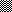
\includegraphics[width=0.5\linewidth]{0config.png}}
    \caption{A $0$-power UPC on a 12-by-12 torus with two stripes}
  \end{subfigure}
  \begin{subfigure}[b]{\linewidth}
    \centering
    \fbox{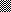
\includegraphics[width=0.5\linewidth]{0config1stripe.png}}
    \caption{A $0$-power UPC on an 11-by-12 torus with one stripe}  
  \end{subfigure}
  \caption{}
\end{figure}



% DIMENSIONS OF POW 0
\par
Thus, 0-power UPCs can be made on any even-by-even or odd-by-even torus.

\par
% UPC OF 1/3 POWER
We will now consider the most interesting of UPCs. % REASONS WHY THEY'RE INTERESTING
\begin{theorem}
\label{13evenThm}
$\frac{1}{3}$-power UPCs must have an equal number of cells of both sides.
\end{theorem}
\begin{proof}
We will count the numbers of cell neighbors of each side. Every cell in a $\frac{1}{3}$-power UPC has two neighbors of each side; two strong and two weak. Thus, no matter how many cells' neighborhoods are counted, there will be equal numbers of strong and weak neighbors. However, each cell has to have been counted four times by all four of its neighbors. Therefore there must be equal numbers of cells of both sides. 

% DEFINE PAIR?
% FINISH PROOF! (COUNT NEIGHBORS OFF)
% 
\end{proof}
\begin{corollary}
UPCs of power $\frac{1}{3}$ cannot exist on boards with an odd number of cells.
\end{corollary}
\begin{corollary}
All $x$-by-$y$ boards where both $x$ and $y$ are odd do not have any $\frac{1}{3}$-power UPCs. 
\end{corollary}
% HYPOTHESIZE INVERSE (CAN BE PROVEN TO EXIST WITH CONSTRUCTION OF 1-STRIPES)
\begin{theorem}
All $x$-by-$y$ grids where $x$ and $y$ are not both odd has at least one $\frac{1}{3}$-power UPC.  
\end{theorem}
\begin{proof}
All boards with at least one even dimension can have a \textit{1-stripe} configuration. The first step in constructing such a configuration is to choose one of the even dimensions. Fill the columns of that dimension with alternating sides. This will form a sequence of columns, with each column being sandwiched between two columns of the opposite side. This ensures that every cell has two neighbors on the opposite side from the adjacent columns, and two neighbors on the same side above and below it in the column.
% CONSTRUCTION!
\begin{example}
% EXAMPLE OF 1-stripes
\begin{figure}[H]
  \centering
  \fbox{
\includegraphics[width=0.5\linewidth]{1-stripes.png}}
  \caption{An example of a 1-stripes configuration on a 16-by-12 torus}
\end{figure}
\begin{remark}
Because of symmetry of side, two opposite configurations can be constructed this way. As well, Boards with two even dimensions will have double the configurations, since they have two choices of dimension to make the columns in. 
\end{remark}
\end{example}
\end{proof}

\par
Here are the empirical data on the numbers of different $\frac{1}{3}$ UPCs for different dimensions.
% TABLE WITH NUMBERS OF 1/3 POWER UPCS OF A GIVEN DIMENSION
% SHOULD I REPLACE THE "-"S WITH 0'S?
\begin{table}[H]
\begin{tabular}{l r | *{9}{r} }
  & & y dimension & & & & & & \\
  & & 2 & 3 & 4 & 5 & 6 & 7 & 8 & & 10\\ \hline
  x dimension & 2 & 1 & 1 & 2 & 1 & 2 & 1 & 2 \\
  & 3 & 1 & - & 1 & - & 2 & - & 1 \\
  & 4 & 2 & 1 & 4 & 1 & 2 & 1 & 5 \\
  & 5 & 1 & - & 1 & - & 1 & - & 1 \\
  & 6 & 2 & 2 & 2 & 1 & 5 & 1 & 2 \\
  & 7 & 1 & - & 1 & - & 1 & - & 1 \\
  & 8 & 2 & 1 & 5 & 1 & 2 & 1 & 18 \\
  & \\
& 10 & & & & & & & & & 28 \\
\end{tabular}
\caption{}
\end{table}
%CONSIDERATIONS OF POSSIBLE DIMENSIONS
The diagonal is of particular interest. At the time of writing, these first 5 terms do not appear in any sequence on the OEIS. \\

\par Figure \ref{All3rd} shows all the constant $\frac{1}{3}$-power configurations for 10-by-10. 

\begin{proposition}
There are three other classes of $\frac{1}{3}$-power UPCs. They are as follows: concentric squares, \textit{staircases}, and exotic. \\
\begin{itemize}
  \item Concentric squares are configurations on $4n$-by-$4n$ tori. They are constructed by tesselating a subconfiguration of concentric squares, alternating sides as you tesselate. This subconfiguration is made by starting with a 2-by-2 square, and alternating sides while adding a border, up to a maximum size of $2n$-by-$2n$.
  \begin{figure}[H]
    \centering
    \fbox{
\includegraphics[width=0.25\linewidth]{ccircles.png}}
  \end{figure}
  \item Staircase configurations involve a continuous path of cells following a repeating pattern of \emph{rights} and \emph{ups}.
  \begin{figure}[H]
    \centering
    \fbox{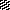
\includegraphics[width=0.25\linewidth]{3rdData10x10_26.png}}
  \end{figure}
  \item Exotic configurations are all other configurations. Not much is known about them. They typically combine squares and paths.
  \begin{figure}[H]
    \centering
    \fbox{
\includegraphics[width=0.25\linewidth]{3rdData10x10_16.png}}
  \end{figure}
\end{itemize}
% ELABORATE

\end{proposition}


\begin{figure}[H]
  \begin{tabular}{ c | c | c | c }
  
\includegraphics[width=0.2\linewidth]{3rdData10x10_1.png} & 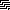
\includegraphics[width=0.2\linewidth]{3rdData10x10_2.png} & 
\includegraphics[width=0.2\linewidth]{3rdData10x10_3.png} & 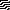
\includegraphics[width=0.2\linewidth]{3rdData10x10_4.png} \\ \hline
  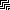
\includegraphics[width=0.2\linewidth]{3rdData10x10_5.png} & 
\includegraphics[width=0.2\linewidth]{3rdData10x10_6.png} & 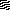
\includegraphics[width=0.2\linewidth]{3rdData10x10_7.png} & 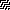
\includegraphics[width=0.2\linewidth]{3rdData10x10_8.png} \\ \hline
  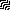
\includegraphics[width=0.2\linewidth]{3rdData10x10_9.png} & 
\includegraphics[width=0.2\linewidth]{3rdData10x10_10.png} & 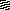
\includegraphics[width=0.2\linewidth]{3rdData10x10_11.png} & 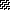
\includegraphics[width=0.2\linewidth]{3rdData10x10_12.png} \\ \hline
  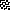
\includegraphics[width=0.2\linewidth]{3rdData10x10_13.png} & 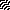
\includegraphics[width=0.2\linewidth]{3rdData10x10_14.png} & 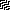
\includegraphics[width=0.2\linewidth]{3rdData10x10_15.png} & 
\includegraphics[width=0.2\linewidth]{3rdData10x10_16.png} \\ \hline
  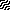
\includegraphics[width=0.2\linewidth]{3rdData10x10_17.png} & 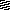
\includegraphics[width=0.2\linewidth]{3rdData10x10_18.png} & 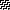
\includegraphics[width=0.2\linewidth]{3rdData10x10_19.png} & 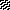
\includegraphics[width=0.2\linewidth]{3rdData10x10_20.png} \\ \hline
  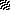
\includegraphics[width=0.2\linewidth]{3rdData10x10_21.png} & 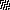
\includegraphics[width=0.2\linewidth]{3rdData10x10_22.png} & 
\includegraphics[width=0.2\linewidth]{3rdData10x10_23.png} & 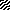
\includegraphics[width=0.2\linewidth]{3rdData10x10_24.png} \\ \hline
  \includegraphics[width=0.2\linewidth]{3rdData10x10_25.png} & \includegraphics[width=0.2\linewidth]{3rdData10x10_26.png} & \includegraphics[width=0.2\linewidth]{3rdData10x10_27.png} & \includegraphics[width=0.2\linewidth]{3rdData10x10_28.png} \\
  \end{tabular}
  \caption{All $\frac{1}{3}$-power UPCs on a 10-by-10 torus}
  \label{All3rd}
\end{figure}


\subsection{The First Iteration} \label{FirstIter}

% PROBLEM: TALK ABOUT WHICH THINGS WE CAN PREDICT FOR THE FIRST ITERATION

\par
This segment is largely about what happens to a grid with a random distribution of cells after a single iteration. This is a valuable simplification because knowing that it has a random distribution allows us to easily use probabilistic methods to consider the dynamics of the game. We consider a random board to be one where each cell has a certain constant probability $p$ of being strong, and a corresponding probability $q=1-p$ of being weak. If $p$ is not specified, we take it to be $0.5$.

% ELABORATE ON RANDOMNESS

\begin{definition}[Subconfiguration Proportion (SP)] % DEFINE AS JUST A TUPLE?
This is a tuple containing the numbers of various subconfigurations.%, and is an element of an SPS. Addition is accomplished by piecewise addition of the counts of the subconfigurations.
% SHOULD THIS BE A FUNCTION FROM SUBCONFIGS TO [0,1]
% element of the above space
\end{definition}


% define higher-order variables (e.g. 2-square proportion, change)
\begin{definition}[Subconfiguration Proportion Space (SPS)]
This is a space of possible subconfiguration proportions.
\end{definition}

\begin{example}
An SPS exists for the proportions of 1-by-2 shapes, counting the incidence of $\mathfrak{w}\mathfrak{w}$, $\mathfrak{w}\mathfrak{s}$, $\mathfrak{s}\mathfrak{w}$, and $\mathfrak{s}\mathfrak{s}$. It has three different subconfigurations, and so is trivially a subset of 
$\{ \left(x,y,z\right) \in [0,1]^3 : x+y+z=1 \}$
\end{example}

%
%  MAKE PICTURES OF TOY EXAMPLES AND CONNECT THEM TO THE TUPLES!
%
%

\begin{example}
$\left( \frac{1}{4} , \frac{3}{4} \right) $ could be a subconfiguration proportion for the SPS of single cells.
 
\end{example}

\begin{definition}[Ratio function]
A ratio operator $R(G)$ is a function from a game $G$ to a subconfiguration proportion. Each SPS has an associated ratio operator.
\end{definition}

\begin{example}
Consider a board with a checkerboard pattern of $\mathfrak{w}$ and $\mathfrak{s}$. The ratio operator for the SPS of individual cells would return $\left(\frac{1}{2},\frac{1}{2}\right)$.
\end{example} % EXPAND EXAMPLE

\begin{definition}[Ratio chain]
A ratio chain is a matrix $C$ representing a markov chain that acts on a subconfiguration proportion vector.
\end{definition}

\begin{proposition}
For any SPS, associated ratio operator $R$, and game $G$, there exists a ratio chain $C$ with associated error distribution $E$ such that
%CR(G)=R(IG)+\vec{\delta}+\vec{\epsilon}
\begin{equation}
	CR\left(G\right)-R\left(IG\right) \sim E
\end{equation}
%where $\vec{\delta}$ and $\vec{\epsilon}$ depend on the the SPS, the size of the game's board, the proportions of the subconfigurations, and how randomized the board is.
%entropy? is this part of the proportions?
% Here, $\vec{\delta}$ represents the random variation due to different boards having the same subconfiguration proportions, whereas $\vec{\epsilon}$ represents any bias the markov chain might have.
%Finally, $n$ represents the number of subconfigurations which compose the configuration.
% switch epsilon and delta?
% OR SHOULD THESE BE DEFINED AS DISTRIBUTIONS?

\end{proposition}
\begin{proof}
You can always make a trivial matrix to do it. Make the diagonal of the matrix the ratios between before and after proportions. This ratio chain would correspond to an error distribution of constant 0.	
\end{proof}
\begin{example}

\end{example}
This leaves us with questions about two things:
\begin{enumerate}
	\item{\textbf{The Ratio Chain:} How can we construct such a ratio chain? Can we approximate it? Is there an optimal construction?}
	\item{\textbf{The Error:} How can we determine the error distribution $E$? Is it possible to minimize it?}
\end{enumerate}

\par
Both of these questions have several approaches. One can determine a ratio chain for a single iteration by simply constructing a matrix which gives the correct before and after SPs. This ratio chain would be pointless and non-predictive since it could only be constructed by knowing empirically what the next iteration would look like. What we would prefer would be to find as general a way to construct a ratio chain: one which requires as little information as possible to successfully predict the dynamics of the SPS for that game.
\par
The first of these questions  % CONTINUE?
\par
The seond question, how to determine the error, is similar to the first insofar as there are different approaches with varying degrees of empiricism. 


% ALGEBRA OUT HOW TO COMPOUND THIS OVER TIME

% HOW THIS CAN BE USED TO SUCCESSFULLY PREDICT THE FIRST ITERATION
\par
There exists a simple and intuitive way to construct a ratio chain for predicting the first iteration of a random board. It involves enumerating all possible neighborhoods of the SPS subconfigurations, and noting down with what proportions certain subconfigurations change into others. This works because the board is randomized, so each neighborhood has an easily calculable probability. The error in this case is a multidimensional binomial distribution. % is it?

\subsubsection{1-square proportion}
\par
A 1-square is equivalent to a single cell. There are two possible states that a 1-square can be in, black or white, $\mathfrak{s}$ or $\mathfrak{w}$. The 1-square proportion is a tuple of the percentages of each state of 1-square on the board.
% definition
% cases
% delta
\par
% FIND THE PROBABILITY THAT A RANDOM CELL CHANGES COLOUR
Consider the closed 2-neighborhood of a cell. Without loss of generality we can fix the centre cell's side. Now, there are $2^{12}$ possible states of this neighborhood. Let $p$ be the proportion of the selected side.
% COME UP WITH BETTER VARIABLE NAMES
\begin{equation}
P(Stay The Same)=\frac{\sum^{12}_{i=0}{\left(Configs with i cells that don't change\right)p^i \left(1-p\right)^{12-i}}}{2^{12}}
\end{equation}
\begin{equation}
P(Change)=1-P(Stay The Same)
\end{equation}
% CONSIDER THE SAMPLING DISTRIBUTION OF THAT PROPORTION WITH THE-NUMBER-OF-CELLS SAMPLES

% instability
\par
Consider the transition probabilities for a 1-square for the first iteration, generated probabilistically. If we consider the proportion of one side, and what it will be in the next iteration, we see that having equal amounts of both sides appears to be an unstable equilibrium. See figure \ref{fig:cellFirst}.
\begin{figure}[H]
	\centering
	\includegraphics[width=\linewidth]{firstIterationCell.png}
	\caption{}
	\label{fig:cellFirst}
\end{figure}
\par 
This is intriguing, because in general (see \ref{LongTermB} for more) having a 50-50 split of sides seems not only to be a stable equilibrium, but a sink to which only the most extreme proportions are not attracted to.

\subsubsection{2-square proportion} \label{2squareFirst}
\par
2-Square subconfigurations are possible states of 2-by-2 squares. There are 16 such subconfigurations, but usually we consider the subconfigurations up to rotational symmetries leaving us with 6 possible states.

\begin{figure}[H]
  \centering
  \begin{subfigure}[b]{0.3\linewidth}
    \fbox{\includegraphics[width=\linewidth]{side.png}}
    \caption{Side}
  \end{subfigure}
  \begin{subfigure}[b]{0.3\linewidth}
    \fbox{\includegraphics[width=\linewidth]{diag.png}}
    \caption{Diagonal}
  \end{subfigure}
  \begin{subfigure}[b]{0.3\linewidth}
    \fbox{\includegraphics[width=\linewidth]{whiteCorner.png}}
    \caption{White Corner}
  \end{subfigure}
  \begin{subfigure}[b]{0.3\linewidth}
    \fbox{\includegraphics[width=\linewidth]{blackCorner.png}}
    \caption{Black Corner}
  \end{subfigure}
  \begin{subfigure}[b]{0.3\linewidth}
    \fbox{\includegraphics[width=\linewidth]{whiteSquare.png}}
    \caption{White Square}
  \end{subfigure}
  \begin{subfigure}[b]{0.3\linewidth}
    \fbox{\includegraphics[width=\linewidth]{blackSquare.png}}
    \caption{Black Square}
  \end{subfigure}
  \caption{2-square states}
\end{figure}

\par
Here are some pictures with various types of subconfigurations coloured.
\begin{figure}[H]
  \centering
  \begin{subfigure}[b]{0.3\linewidth}
    \fbox{\includegraphics[width=\linewidth]{img0019Coloured2.png}}
    \caption{Sides}
  \end{subfigure}
  \begin{subfigure}[b]{0.3\linewidth}
    \fbox{\includegraphics[width=\linewidth]{img0019Coloured3.png}}
    \caption{Diagonals}
  \end{subfigure}
  \begin{subfigure}[b]{0.3\linewidth}
    \fbox{\includegraphics[width=\linewidth]{img0019Coloured5.png}}
    \caption{White Corner}
  \end{subfigure}
  \begin{subfigure}[b]{0.3\linewidth}
    \fbox{\includegraphics[width=\linewidth]{img0019Coloured4.png}}
    \caption{Black Corner}
  \end{subfigure}
  \begin{subfigure}[b]{0.3\linewidth}
    \fbox{\includegraphics[width=\linewidth]{img0019Coloured0.png}}
    \caption{White Squares}
  \end{subfigure}
  \begin{subfigure}[b]{0.3\linewidth}
    \fbox{\includegraphics[width=\linewidth]{img0019Coloured1.png}}
    \caption{Black Squares}
  \end{subfigure}
  \caption{2-square samples from a 12-by-12 torus simulation}
\end{figure}

\par
If we have a random board, then we can easily consider what the starting proportions of these subconfigurations should be. 
\begin{table}[H]
\begin{tabular}{r | l}
  Shape & Expected Starting Proportion \\ \hline
  Side & $\frac{1}{4}$ \\
  Diagonal & $\frac{1}{8}$ \\
  White Corner & $\frac{1}{4}$ \\
  Black Corner & $\frac{1}{4}$ \\
  White Square & $\frac{1}{16}$ \\
  Black Square & $\frac{1}{16}$ \\
\end{tabular}
\caption{}
\end{table}

\par
The problem now is to predict what the proportions of these 6 subconfigurations will be in the next iterations. To accomplish this, we will construct a ratio chain. To construct this chain:
\begin{enumerate}
  \item{} Consider the 2-neighborhood around a 2-square
  \begin{figure}
    \caption{2-neighborhood}
  \end{figure}
  \item{} For all 6 different subconfigurations:
  \begin{enumerate}
    \item{} For all $2^{20}$ possible neighborhoods:
    \begin{enumerate}
      \item{} Place the subconfiguration in the centre of the neighborhood.
      \item{} Iterate once.
      \item{} Record which subconfiguration is now in the centre.
    \end{enumerate}
    \item{} Divide the counts of the final subconfigurations by $2^{20}$ to normalize them.
  \end{enumerate}
  
\end{enumerate}

%huge section
\subsection{Long Term Behaviour}
\label{LongTermB}
% HAVE BLURB ABOUT WHY LONG-TERM
\par
There are many reasons why we should consider the long-term behaviour of the game. The first being that it represents an averaged or compounded version of the game rules. 
\par
It is also about local versus global structure!

% PICTURES OF BEFORE AND AFTER

\subsubsection{Threshold for Homogeneous Stability} \label{HomoStability}
% DEFINE HOMOGENEOUS STABILITY?
\par
Recall from \ref{SpecialShapes} that the L, I, and O tetrominoes are parastable. These are the smallest parastable patterns. By the nature of their parastability, they can "re-seed" a grid with very few of a given side. Thus, we can make a probabilistic argument for the cutoff below which the proportion between strong and weak should not be able to return to 50/50.

\par
These three types of tetrominoes have 11 different configurations, because of their symmetries.
% PUT IN OTHER PARAGRAPH?
\par
Let $X$ be the number of parastable tetrominoes on a torus with
width $n$ and height $m$, and $\{X_{i,j}:i\in\{1,\ldots,n\},j\in\{1,\ldots,m\}\}$
be the indicator variables for there being a parastable tetromino at
position $\left(i,j\right)$. Finally, let $p$ be the proportion of cells
on the torus with the given side. Then
\begin{equation}
	E(X_{i,j})=11p^4
	\end{equation}
And so by linearity of expected value
\begin{equation}
	E(X)=\sum_{i=1}^n \sum_{j=1}^m E(X_{i,j})=\sum_{i=1}^n \sum_{j=1}^m 11p^4 = 11nmp^4
\end{equation}
Thus, the critical proportion such that we expect there to be one
parastable tetromino is $p=\left(\frac{1}{11nm}\right)^{\frac{1}{4}}$

\begin{figure}[H]
  \centering
  \begin{subfigure}[b]{0.6\linewidth}
    \fbox{\includegraphics[width=\linewidth]{homostableData25x25x25.png}}
    \caption{25-by-25 torus. Expected crossover at ${p=\frac{1}{11\times25\times25}}^{\frac{1}{4}}=0.110$}
  \end{subfigure}
  \begin{subfigure}[b]{0.6\linewidth}
    \fbox{\includegraphics[width=\linewidth]{homostableData50x50x25.png}}
    \caption{50-by-50 torus. Expected crossover at ${p=\frac{1}{11\times50\times50}}^{\frac{1}{4}}=0.077$}
  \end{subfigure}
  \begin{subfigure}[b]{0.6\linewidth}
    \fbox{\includegraphics[width=\linewidth]{homostableData100x100x25.png}}
    \caption{100-by-100 torus. Expected crossover at ${p=\frac{1}{11\times100\times10}}^{\frac{1}{4}}=0.055$}
  \end{subfigure}
  \caption{}
\end{figure}

\subsubsection{Behaviour of Power} \label{Power}

The power of a grid usually increases over time to approach an asymptote. 

\subsubsection{1-2 and 2-2 Proportions} \label{LongTerm2P}
%Show why 3-3 not as important via entropy
%TALK ABOUT WHY IT IS INTERESTING THAT THE PROPORTIONS ARE THE SAME FOR RANDOM SEEDS AND PARASTABLE STARTS

\par
This segment deals with 

\begin{definition}[$n$-$m$ proportion]
This is the proportions of the different configurations of an $n$ by $m$ rectangle.
\end{definition}

\begin{figure}[H]
  % MAKE THE TITLES ON THIS GRAPH LARGER!
  \includegraphics[width=\linewidth]{shapesdata300x300(rand).png}
  \caption{2-square proportions on a 300-by-300 torus over time}
\end{figure}

\begin{table}[H]
\begin{tabular}{r|l}
  Shape & Final Proportion \\ \hline
  Side & 0.334 \\
  Diagonal & 0.020 \\
  White Corner & 0.188 \\
  Black Corner & 0.188 \\
  White Square & 0.135 \\
  Black Square & 0.135 \\  
\end{tabular}
\end{table}

\par
The variables of 1-2 and 2-2 proportion are intriguing because they directly disprove the hypothesis that the distribution of large subconfigurations is predictable by their smaller subsubconfigurations' proportions. % REWRITE THIS LINE?


% TALK ABOUT HOW MUCH IT DID WORK AND HOW MUCH IT DIDN'T
\par
Recall the ratio chain used to model the proportion of 2-squares in section \ref{2squareFirst}. If we apply this ratio chain continuously, we arrive at the following stable state:
\begin{table}[H]
\begin{tabular}{r|l}
  Shape & Ratio Chain Stable State Proportion \\ \hline
  Side & 0.122 \\
  Diagonal & 0.006 \\
  White Corner & 0.116 \\
  Black Corner & 0.116 \\
  White Square & 0.320 \\
  Black Square & 0.320 \\
\end{tabular}
\caption{}
\end{table}
% SHOULD I PLACE THE OTHER DATA BESIDE THIS?

\par
If we compare these data to the empirical long-term proportions, we get some mixed results.

\begin{table}[H]
\begin{tabular}{r|c c c | l}
  Shape & Actual Starting & Actual Final & Ratio Chain Final & Final Error \\ \hline
  Side & 0.250 & 0.334 & 0.122 & -0.212 \\
  Diagonal & 0.125 & 0.020 & 0.006 & -0.014 \\
  White Corner & 0.250 & 0.188 & 0.116 & -0.072 \\
  Black Corner & 0.250 & 0.188 & 0.116 & -0.072 \\
  White Square & 0.062 & 0.135 & 0.320 & 0.185 \\
  Black Square & 0.062 & 0.135 & 0.320 & 0.185 \\
\end{tabular}
\end{table}
\par The first thing that you will notice is that the ratio chain gets the long-term proportions significantly wrong. However, there is also an interesting trend. With the exception of sides, every proportion moves "in the right direction". Diagonals decrease significantly, and the ratio chain reflects this. The corners decrease slightly, and the ratio chain reflects this. The squares increase significantly, and the ratio chain reflects this. In all these cases, the ratio chain appears to simply \textit{overshoot} its target.

\subsubsection{Stability Over Time}
The number of cells that changed in the last iteration decreases over time, towards an asymptote.

\begin{figure}[H]
  \centering
  \includegraphics[width=0.75\linewidth]{changeProps.png}
  \caption{}
\end{figure}

\subsubsection{Cycle length}

\begin{figure}[H]
  \includegraphics[width=\linewidth]{precycles.png}
  \caption{Precycle length for random $n$-by-$n$ boards where $5\leq n \leq 100$}
\end{figure} % MENTION HOW THE LINE OVERESTIMATES AT THE SMALL VALUES?

\par
There's an argument here for why the global structure of the game cannot be determined by just the local structure of the game. This is because if the only the local structure mattered, then the precycle length shouldn't be increasing (at all? linearly? should it approach an asymptote?).

\subsubsection{The Search for Entropy}

\subsection{Some other results}

%Spectrum stuff
%Crystalization (parastability breaking down at 50%-prob-of-changing)
%change space
%transition matrix images

\section{Conclusion}

In conclusion, 

\subsection{Open Problems}
\begin{itemize}
\item
Enumerating all $\frac{1}{3}$ - power stable configurations. This is equivalent to the general problem of colouring cells on a torus such that each cell has two neighbors of each colour. (see \ref{UPCs})
\item
Enumerating all stable subconfigurations on an empty grid (see \ref{EmptyGrid}).
\item
Variance of the threshold for homogeneous stability. (see \ref{HomoStability})
\item
Proof for maximum average power. (see \ref{Power})
\item
Method of constructing a ratio-chain for long-term behaviour. (see \ref{LongTerm2P})
\end{itemize}
% TODO BIBLIOGRAPHY? DO I HAVE SOURCES?

\subsection{Acknowledgments}

\end{document}
